\section{Deep learning}
Die Begriffe \textit{Deep Learning}, \textit{maschinelles Lernen} und, \textit{künstliche Intelligenz}, werden oft fälschlicherweise auswechselbar verwendet, und in eine Schublade geräumt. Es gibt allerdings eine ganz klare, und für das Verständnis wichtige Hierarchie zwischen den Wörtern. Um Klarheit zu verschaffen werden darum alle Gebiete aufgeführt.

\begin{figure}[hbt]
	\centering
		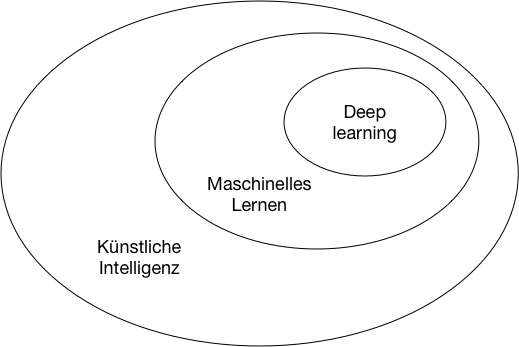
\includegraphics[width=0.6\textwidth]{assets/hierarchy.png}
	\caption{Künstliche Intelligenz, Maschinelles Lernen und Deep Learning}
	\label{img:hierachy}
\end{figure}

Das Gebiet der künstlichen Intelligenz gibt es schon so lange wie den Computer selbst. Die Frage, wie schlau ein Computer werden kann, beschäftigt uns bis heute. Als anerkannte Definition für KI gilt, das Bestreben, intellektuelle Aufgaben, die normalerweise von Menschen gelöst werden, zu automatisieren.

Erste Erfolge erreichte man zum Beispiel mit Schachcomputern, die handgeschriebene Regeln befolgten. Diese Form von künstlicher Intelligenz hatte aber schnell Grenzen, da viele Prozesse schlicht zu komplex waren, um sie unter angemessenem Aufwand mit Regeln zu beschreiben. Aus dieser Idee entwickelte sich das Konzept des maschinelles Lernens.

Der Ablauf von maschinellem Lernen ist grundlegend anders als konventionelles Programmieren. Der Entwickler muss  keinen Programmcode mit festen Regeln schreiben, im Gegenteil. Man liefert dem Computer Eingabe und Ausgabe, und der Computer lernt die Regeln selbst. Maschinelles Lernen entstand blühte erst in 90'er Jahren auf, wurde aber schnell zum grössten Teilgebiet der künstlichen Intelligenz.

Beim maschinellem Lernen, lernt die Software im Grunde eine nützlichere Darstellungsweise der Daten bzw. der Eingabe. Anhand dieser anderen Darstellungsweise kann der Computer die Antwort einfach erkennen. Wenn der Computer stufenweise nützlichere Repräsentationen bestimmt, kann er zunehmend komplexe Probleme in einfachere Zwischenschritten lösen. Genau das ist deep learning. Es beschreibt also mehr das Konzept von stufenweisem Lernen als eine Methode selber. Ein weit verbreitete Mehode sind allerdings \textit{tiefe künstliche neuronalen Netzen}.\parencite[vgl.][]{chollet}

\subsection{Künstliche Neuronale Netze}

\textit{Künstliche neuronale Netze} hat man sich, wie der Name schon preisgibt, von der Natur abgesehen. Ähnlich wie in unserem Gehirn gibt es Neuronen bzw. Knoten und dazwischenliegende Verbindungen. Die Verbindungen haben ein Gewicht $w$. Künstliche Neurone Netze haben sich aber mittlerweile so stark weiterentwickelt, dass sie nebst der ursprünglichen Idee, nichts mehr mit der Natur zu tun haben. \\

Der Wert eines Knotens ist eine Funktion der Summe all er seiner eingehenden Verbindungen. Diese Funktion wird Aktivierungsfunktion $\sigma$ genannt. Die Aktivierungsfunktion ist wichtig damit das Netwerk auch nicht lineare Repräsentationen lernen kann. Eine bekannte Aktivierungsfunktion ist zum Beispiel die \textit{RELU} Funktion. \parencite{neuronale_netze} 
$$\sigma(x) = relu(x) = \text{max}(0, x)$$

Der Wert einer eingehenden Verbindung ist errechnet sich aus dem Produkt des Gewichts $w$ und dem Wert des ausgehenden Knotens. Wenn man alles zusammensetzt ergibt sich für den Wert irgendeinen Knotens $o$ mit Vorgänger Knoten $h$ diese Formel:
$$ o = \sigma\Big(\sum_i h_i \cdot w_{i}\Big)$$
Mit dieser Formel propagieren sich die Werte der Anfangsknoten durch das ganze Netzwerk. Um das Prinzip anschaulicher zu machen, wird ein Beispiel-Durchlauf vorgeführt. Die verwendeten Gewichte sind willkürlich.

Die Aufgabe des vorgestellten Netzwerks könnte zum Beispiel sein, zwischen Hund und Katze zu unterscheiden. Die Eingaben $x_1$ und $x_2$ würden dann gewisse Merkmale des Tieres beschreiben. 1 würde heissen das Tier besitzt das Attribut und 0 das Gegenteil. Die Ausgabe $o$ wäre dann die Wahrscheinlichkeit, dass das Tier eine Katze ist.

\begin{figure}[hbt]
	\centering
		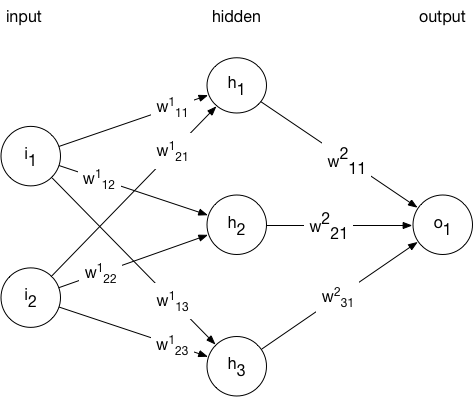
\includegraphics[width=0.9\textwidth]{assets/neural_net.png}
	\caption{Grafische Darstellung eines künstlichen neuronalen Netzwerks anhand eines Beispiels}
	\label{img:neuralnet}
\end{figure}

Die mathematischen Operationen in einem neuronalen Netwerk lassen sich alle als Matrizen-Operationen berechnen. Mit Matrizen kann der Computer auf einer Grafikkarte und mit einem BLAS (\textit{Basic linear algebra system}) sehr effizient rechnen \parencite{neuronale_netze} .

Was bis jetzt berechnet wurde nennt man den \textit{Vorwärtspass}. Aus einer Eingabe wurde die Ausgabe berechnet. Daran war aber noch nichts intelligent. Erst jetzt können die Parameter der Funktion, die Gewichte, aus diesem Beispiel lernen. Um diese zu verbessern braucht es eine \textit{Verlust Funktion} die uns angiebt, wie weit die Ausgabe vom korrekten Ziel entfernt ist. Wenn man in unserem Beispiel davon ausgeht, dass die Eingabe wirklich zu einer Katze gehört, wäre so etwas möglich:
$$ \text{Verlust}(output, target) = |target-output| = |1.0-0.747| = 0.253$$
Anhand des Verlustwerts passt das Netzwerk die Gewichte schrittweise an. Diesen Teil übernimmt der  \textit{Optimierer}. Ein einfacher Optimierer ist zum Beispiel das Gradientenverfahren \parencite{gradient}.

\begin{figure}[hbt]
	\centering
		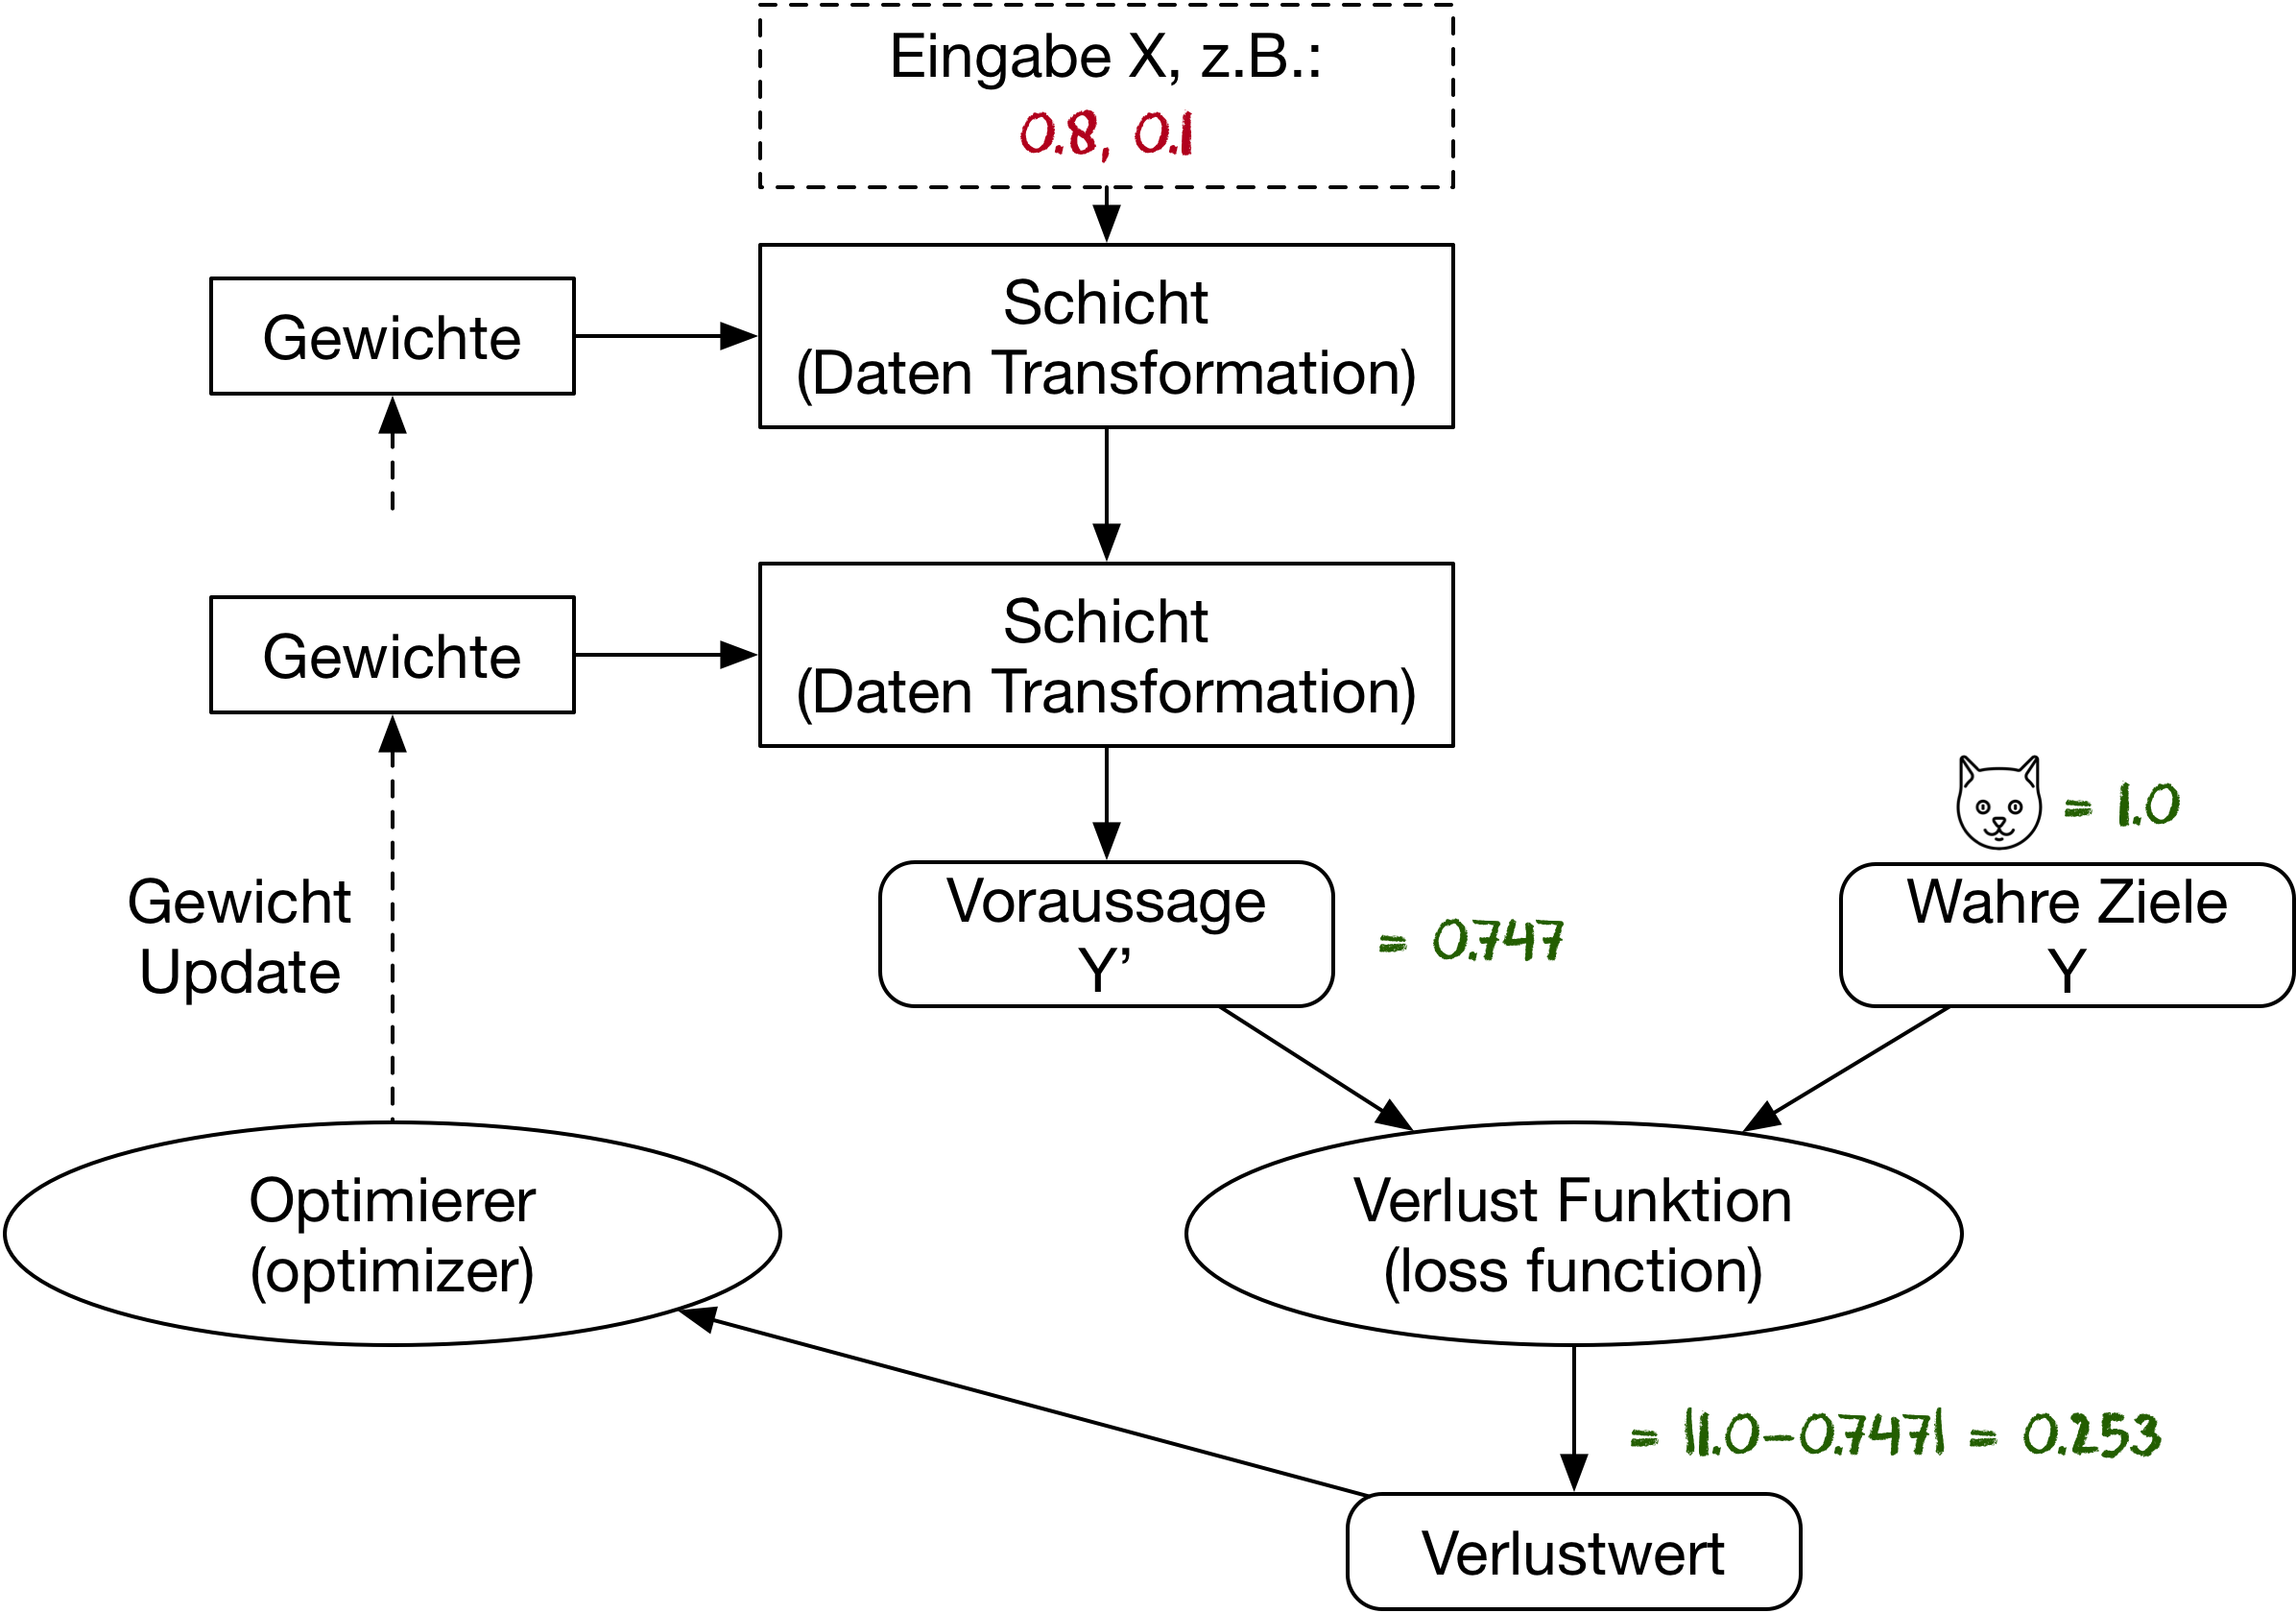
\includegraphics[width=0.8\textwidth]{assets/anatomy.png}
	\caption{Grafische Darstellung des Lern-Prozesses anhand eines Beispiels}
	\label{img:anatomy}
\end{figure}

Da bei diesem Typ von neuronalen Netzwerken alle Knoten miteinander verbunden sind, wird es oft \textit{dense neural network} genannt.
Es ist bewiesen dass solche neuronale Netze jede Funktion abbilden können\parencite[][Kap. 4]{universal}.


\subsection{Convolutional Neural Networks}
\textit{Convolutional Neural Networks} sind eine sehr weit verbreitete Methode im Feld von \textit{Computer Vision}. Der fundamentale Unterschied zwischen dem oben besprochenen \textit{dense network} und einem \textit{CNN} ist, dass ein \textit{CNN} lokale Muster erkennen kann, wo hingegen das vorherige Netzwerk nur globale Muster erkennen konnte. Das heisst, dass ein Muster an einer bestimmten Stelle angetroffen wird, an jeder anderen Stelle ebenfalls erkannt wird. \parencite{chollet}

Um das zu erlauben, teilen gewisse Verbindungen das gleiche Gewicht. In Abbildung \ref{img:conv} (Oberer Teil) sind das die gleichfarbigen Verbindungen. Weniger Gewichte führen zusätzlich dazu, dass das Netzwerk schneller lernen kann.
\begin{figure}[hbt]
	\centering
		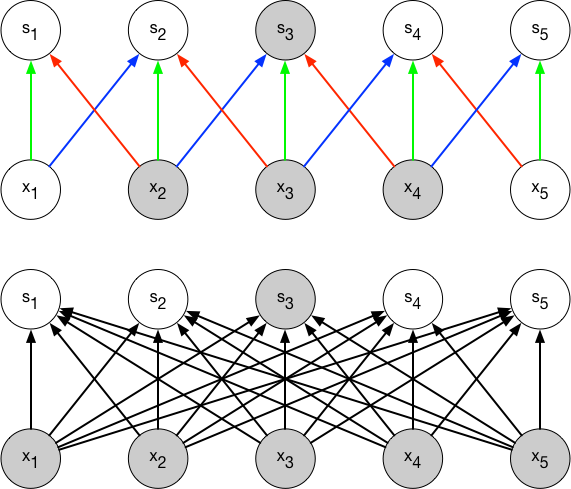
\includegraphics[width=0.6\textwidth]{assets/conv_1d.png}
	\caption{(\textit{Oben})1D Convolution mit \textit{kernel} der Grösse 3. $s_3$ wird durch 3 inputs beeinflusst.
		     (\textit{Unten}) \textit{Dense Network}. $s_3$ wird durch alle inputs beeinflusst.\parencite{goodfellow}}
	\label{img:conv}
\end{figure}

Ein weiterer Vorteil von \textit{Convolutional neural networks} ist, dass sie eine räumliche Hyrarchie von Mustern erlernen können. Wenn die Eingabe das Bild einer Katze ist, wird zum Beispiel die erste Schicht unterschiedliche Kanten erkennen, die zweite Schicht dann einzelne Merkmale (z.b Augen), und so weiter.

Damit das gilt, muss aber der analysierte Bereich eines Knotens, von Schicht zu Schicht grösser werden. Deshalb wird meisten nach jedem \textit{convolution layer} ein \textit{pooling layer} gesetzt. Das \textit{pooling layer} fasst mehrere Datenpunkte zusammen um dem nächsten Netzwerk eine grösseren Analysebereich zu verschaffen.
\begin{figure}[hbt]
	\centering
		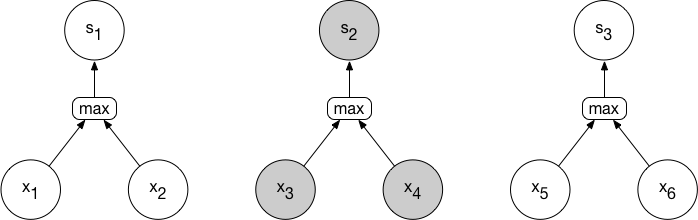
\includegraphics[width=0.6\textwidth]{assets/pooling_1d.png}
	\caption{Abbildung eines 1D Max-Pooling layer. $s_2$ ist $\max (x3, x4)$}
	\label{img:pool}
\end{figure}


\subsection{Recurrent Neural Networks}
Eine gemeinsame Eigenschaft von allen \textit{dense neural networks} und CNN's ist, dass sie keinen Speicher haben. Bei jedem Vowärtspass berechnet das Netzwerk alles von neuem ohne Erinnerungen an vorherige Durchläufe. Dieses Verhalten ist das absolute Gegenteil vom menschlichem Denkprozess. Wenn wir einen Satz lesen, durchgehen wir ihn Wort nach Wort und merken uns den vorherigen Kontext.

\textit{Recurrent Neural Networks} (RNN) bilden diesen Prozess vereinfacht nach. Sie besitzen eine interne wiederkehrende Schleife die dem Netzwerk Informationen aus dem vorherigen Durchlauf bereitstellt (Siehe Abbildung \ref{img:rnn_loop}). Die RNN Zelle berechnet dann die nächste Ausgabe sowohl aus der neuen Eingabe wie auch mit den Erinnerungen der letzten Ausgabe. \parencite{chollet}\\
\begin{figure}[hbt]
	\centering
		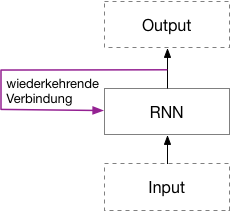
\includegraphics[width=0.25\textwidth]{assets/rnn_loop.png}
	\caption{RNN mit Schlaufe}
	\label{img:rnn_loop}
\end{figure}

Der Vorgang lässt sich grafisch über die Zeit aufgerollt darstellen (Abbildung \ref{img:rnn_unrolled}). In dieser Darstellung fällt auf, dass das Netzwerk theoretisch für jeden Schritt eine Ausgabe besitzt. Die zwischenliegenden Ausgaben sind vor allem wichtig wenn man eine weitere Schicht an das Netzwerk anhängen will. Sonst behält man meist nur die letze Ausgabe, da diese indirekt Informationen über alle anderen beinhaltet.\\
\begin{figure}[hbt]
	\centering
		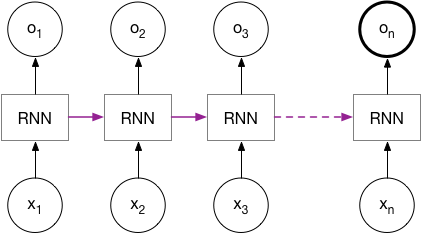
\includegraphics[width=0.67\textwidth]{assets/rnn_unrolled.png}
	\caption{RNN aufgerollt über die Zeit}
	\label{img:rnn_unrolled}
\end{figure}

Das ganze Prinzip ergibt jedoch nur Sinn, wenn frühere Eingaben tatsächlich einen Einfluss auf spätere Ausgaben haben. Eine praktische Anwendung ist das Verarbeiten von zeitlichen Sequenzen wie Wetterdaten und Sprache. Die einzelnen Lernbeispiele werden nach zeitlich zerteilt und stückweise dem Netzwerk gefüttert.
Eine fortgeschrittene Implementation von RNN Zellen ist unter anderem die \textit{Long short-tem memory} (LSTM) Zelle \parencite{schmidhuber}. Durch das einführen von unterschiedlichen wiederkehrenden Verbindungen wird verhindert, dass ältere Signale langsam verschwinden \parencite{chollet}.
\subsection{Generational Adversial Neural Networks}